% figures of the spectras

% figure Spectra_Si.png
\begin{figure}
    \centering
    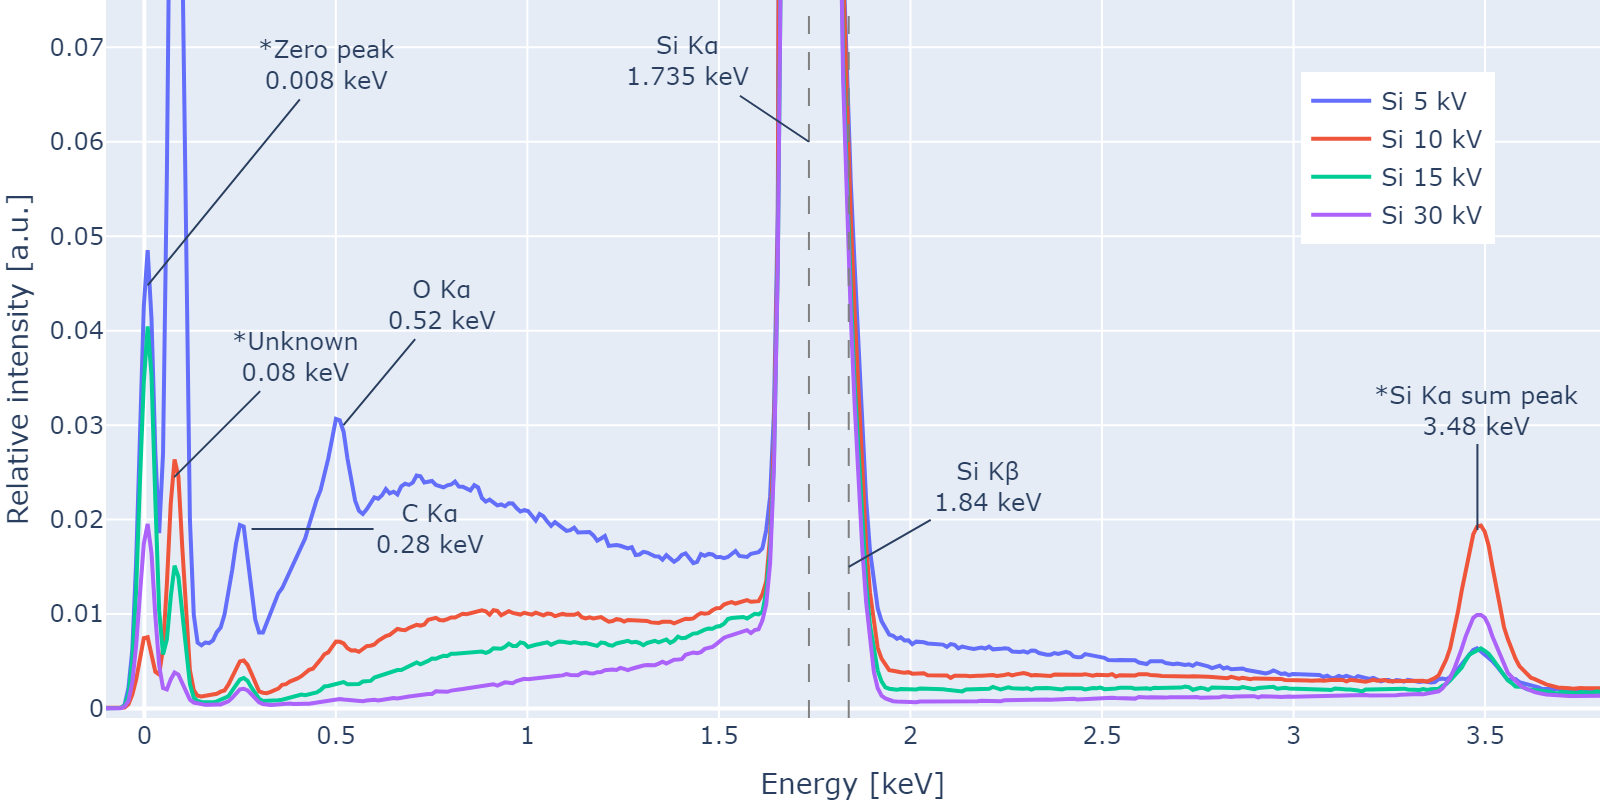
\includegraphics[width=0.90\textwidth]{../eds-analysis/plots/spectra_plots/Si_everything.png}
    \caption{
        The spectra of the pure Si wafer sample part.
        All four spectra have one large peak at 1.73 keV, which is the Si K$\alpha$ peak with some signal at the K$\beta$ peak at 1.83 keV.
        The relative weight for Si K$\beta$ to K$\alpha$ is 0.028.
        The zero peak is marked at 0.008 keV.
        After the zero peak there is another sharp peak at 0.080 keV, which is not identified.
        The energies annotated are the end of the annotation line, which can deviate a few percent from the actual peak energy.
    }
    \label{fig:results:Spectra_Si}
\end{figure}

% figure Spectra_Al.png
\begin{figure}
    \centering
    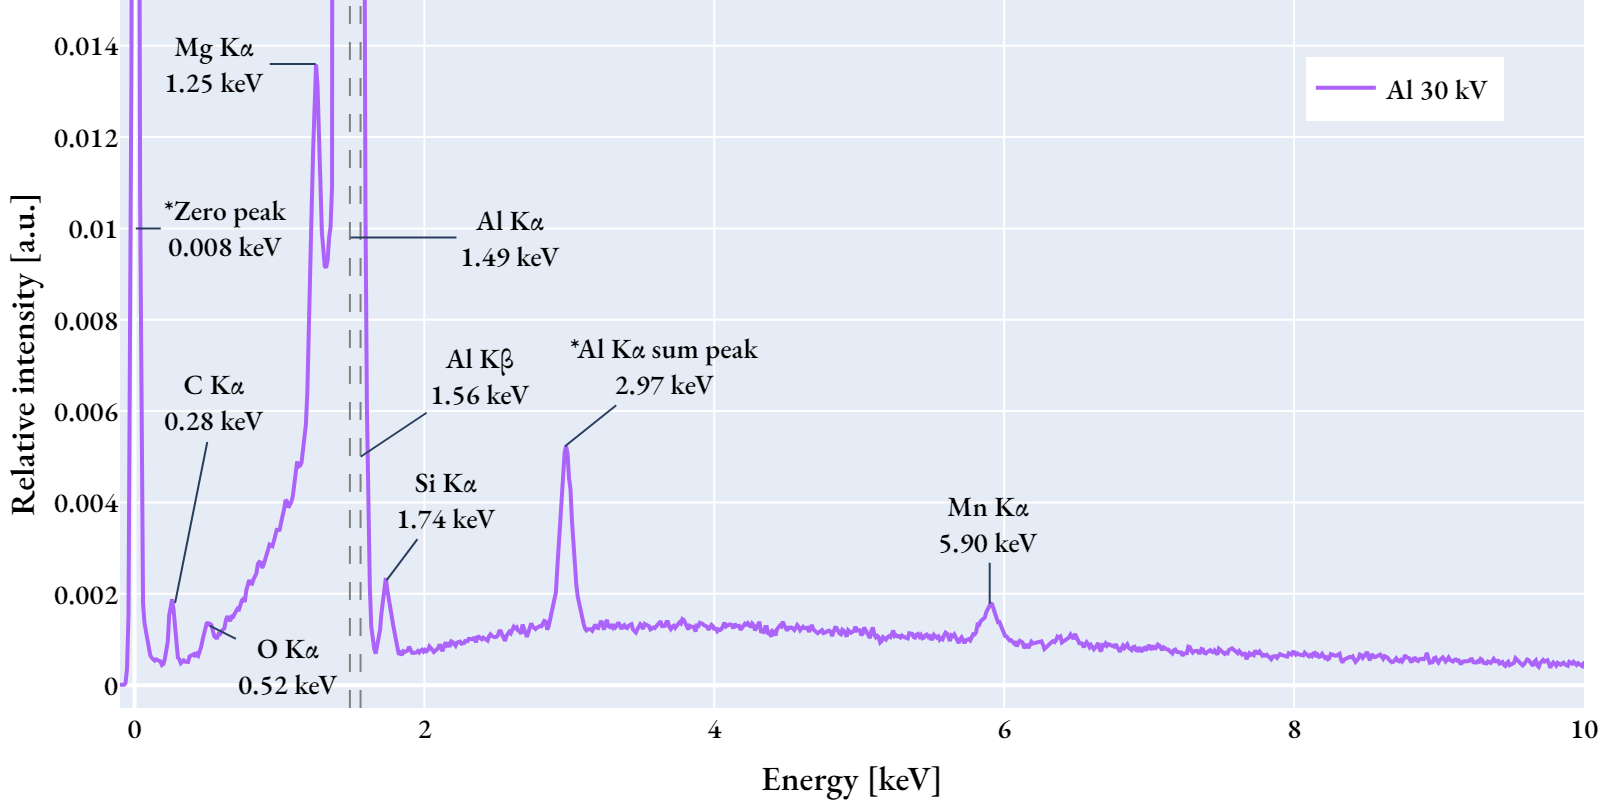
\includegraphics[width=0.90\textwidth]{../eds-analysis/plots/spectra_plots/Al_everything.png}
    \caption{
        The spectra of the Al sample part.
        This was expected to be Fe, thus the label is wrong.
        The peak at 1.49 keV is the Al K$\alpha$ peak with some signal at the K$\beta$ peak at 1.56 keV.
        The relative weight for Al K$\beta$ to K$\alpha$ is 0.013 (from HyperSpy).
        Fe K$\alpha$ at 6.40 keV has a question mark, because the FIB stub was initially expected to be Fe.
        The signal from Fe K$\alpha$ is barely a signal different than the background.
    }
    \label{fig:results:Spectra_Al}
\end{figure}

% figure Spectra_Cu.png
\begin{figure}
    \centering
    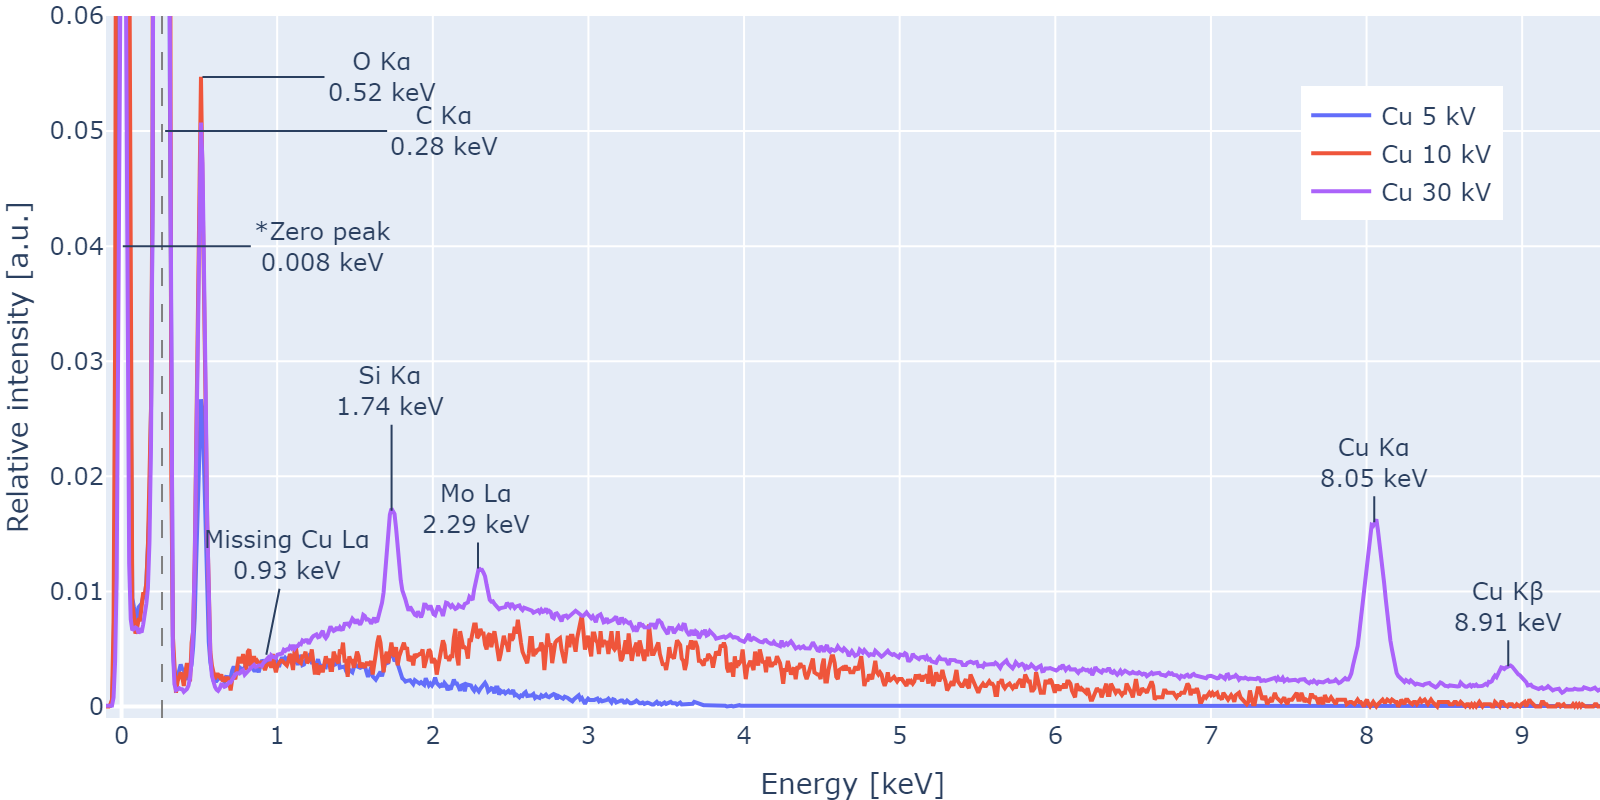
\includegraphics[width=0.90\textwidth]{../eds-analysis/plots/spectra_plots/Cu_everything.png}
    \caption{
        The spectra of the Cu sample part.
        The Cu sample was Cu-tape from the lab, but the Cu K$\beta$ peak is only barely visible at the 30 kV spectrum.
        The highest peak in all three spectra is at 0.260 keV, which is the C K$\alpha$ peak, slightly off from the expected 0.277 keV.
        The plot is limited to 9.5 keV, because there are no peaks above that energy.
        The Mo L$\alpha$ peak at 2.29 keV is visible at the 30 kV spectrum, but not in the 5 or 10 kV spectra.
        The Mo L$\alpha$ is marked with a question mark, because there are no signal whatsoever at the Mo K$\alpha$ peak at 17.48 keV.
        The peaks which are taller than the plot is marked with a vertical grey stippled line.
    }
    \label{fig:results:Spectra_Cu}
\end{figure}

% figure Spectra_GaAs.png
\begin{figure}
    \centering
    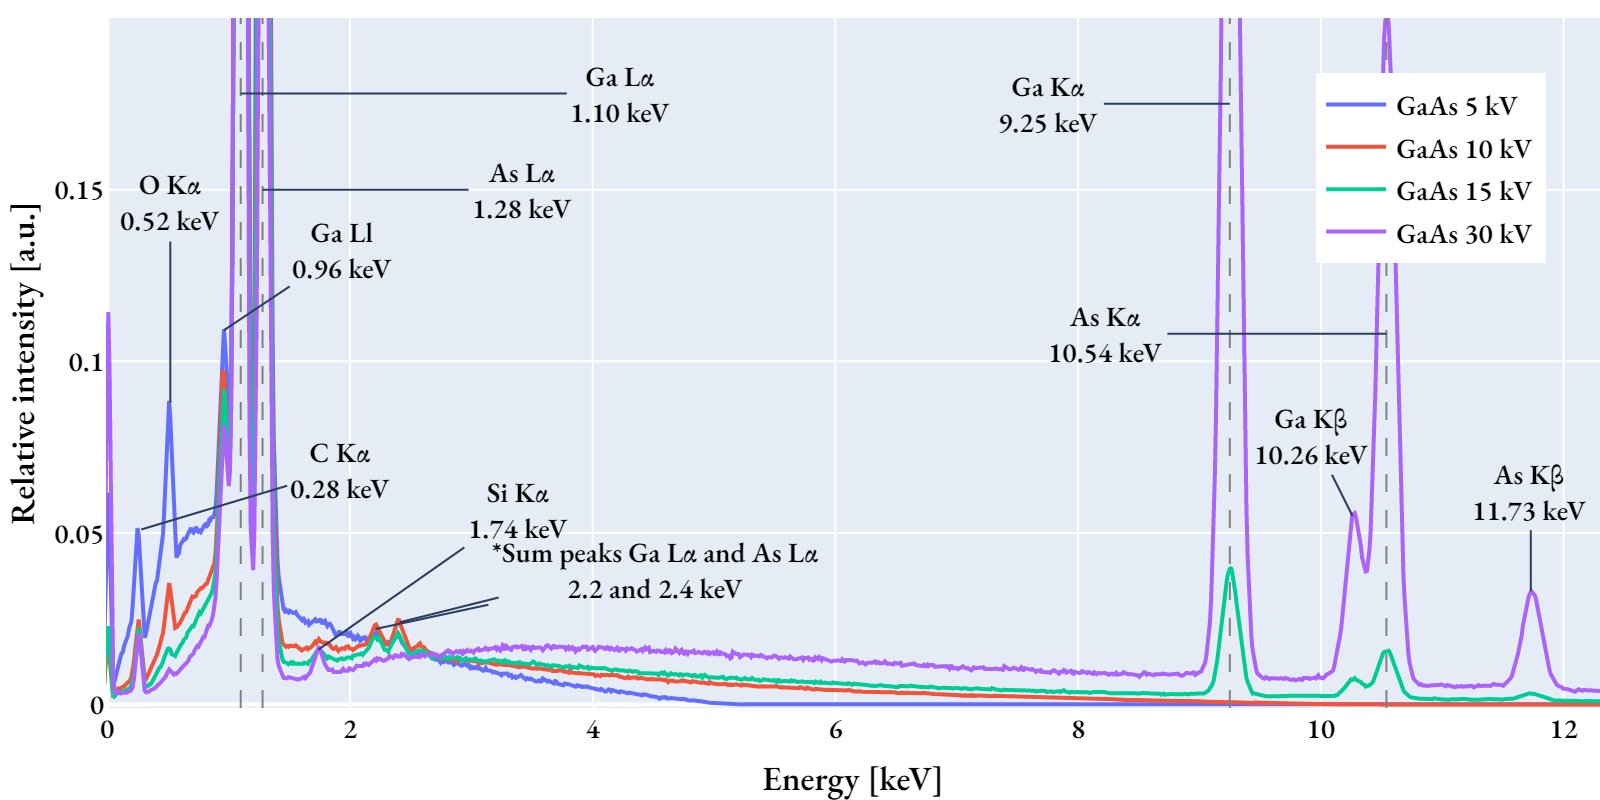
\includegraphics[width=0.90\textwidth]{../eds-analysis/plots/spectra_plots/GaAs_everything.png}
    \caption{
        The spectra of the GaAs sample part.
        Both the K-peaks and the L-peaks of Ga and As are visible.
        There is a peak at 0.511 keV, which is the O K$\alpha$ peak.
        There is a peak at 0.260 keV, which is the C K$\alpha$ peak.
    }
    \label{fig:results:Spectra_GaAs}
\end{figure}


% figure Spectra_GaAs.png
\begin{figure}
    \centering
    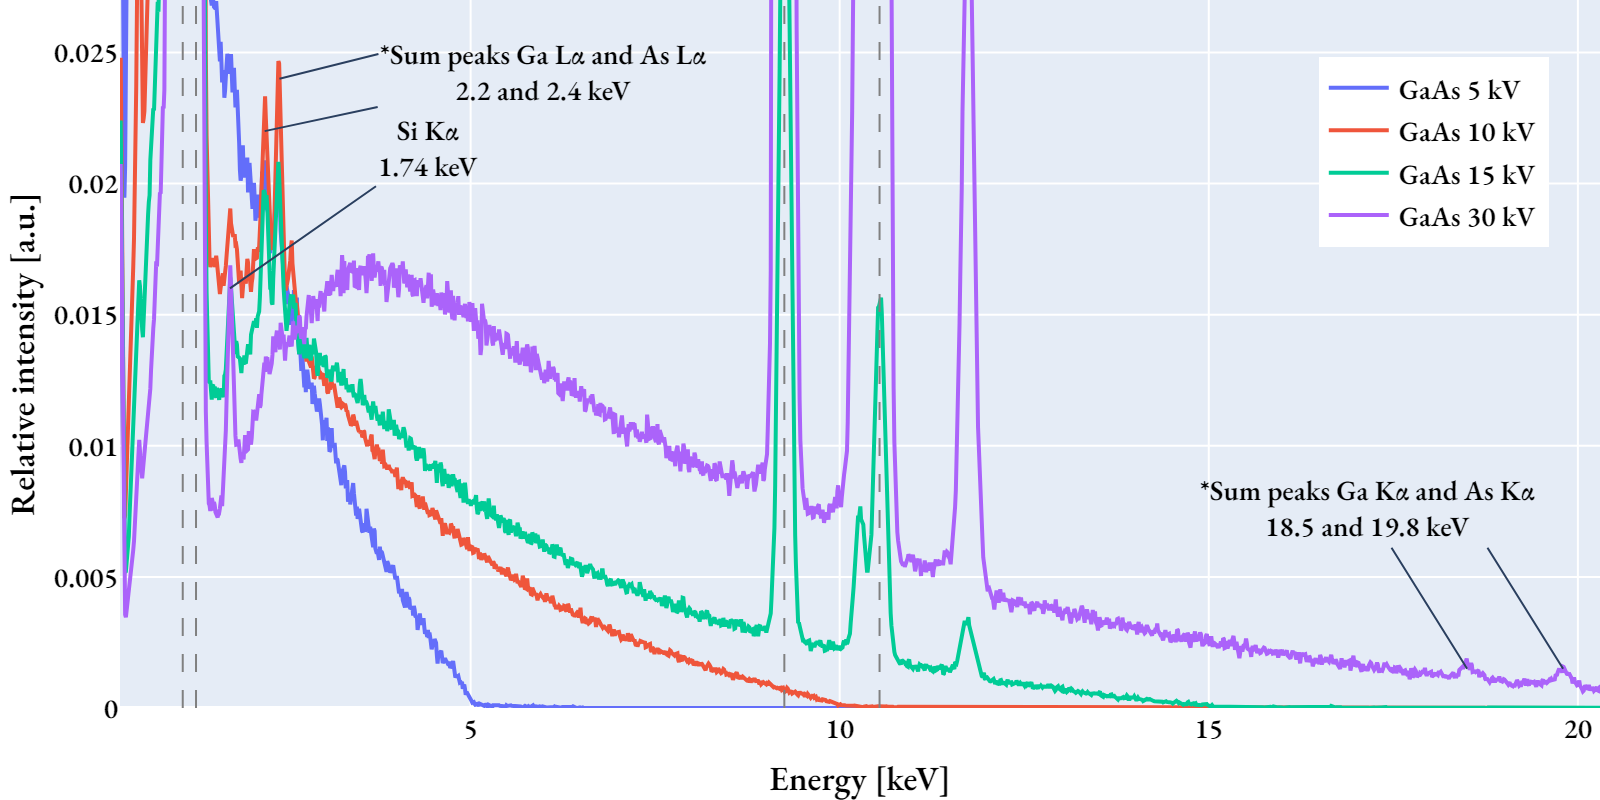
\includegraphics[width=0.90\textwidth]{../eds-analysis/plots/spectra_plots/GaAs_bg_and_sum_peaks.png}
    \caption{
        A zoomed in view of the GaAs sample part.
        The background is easier to see, and the sum peaks are visible.
        The sub peaks are on \brynjar{Add energies!}
    }
    \label{fig:results:Spectra_GaAs}
\end{figure}

% figure Spectra_Mo.png
\begin{figure}
    \centering
    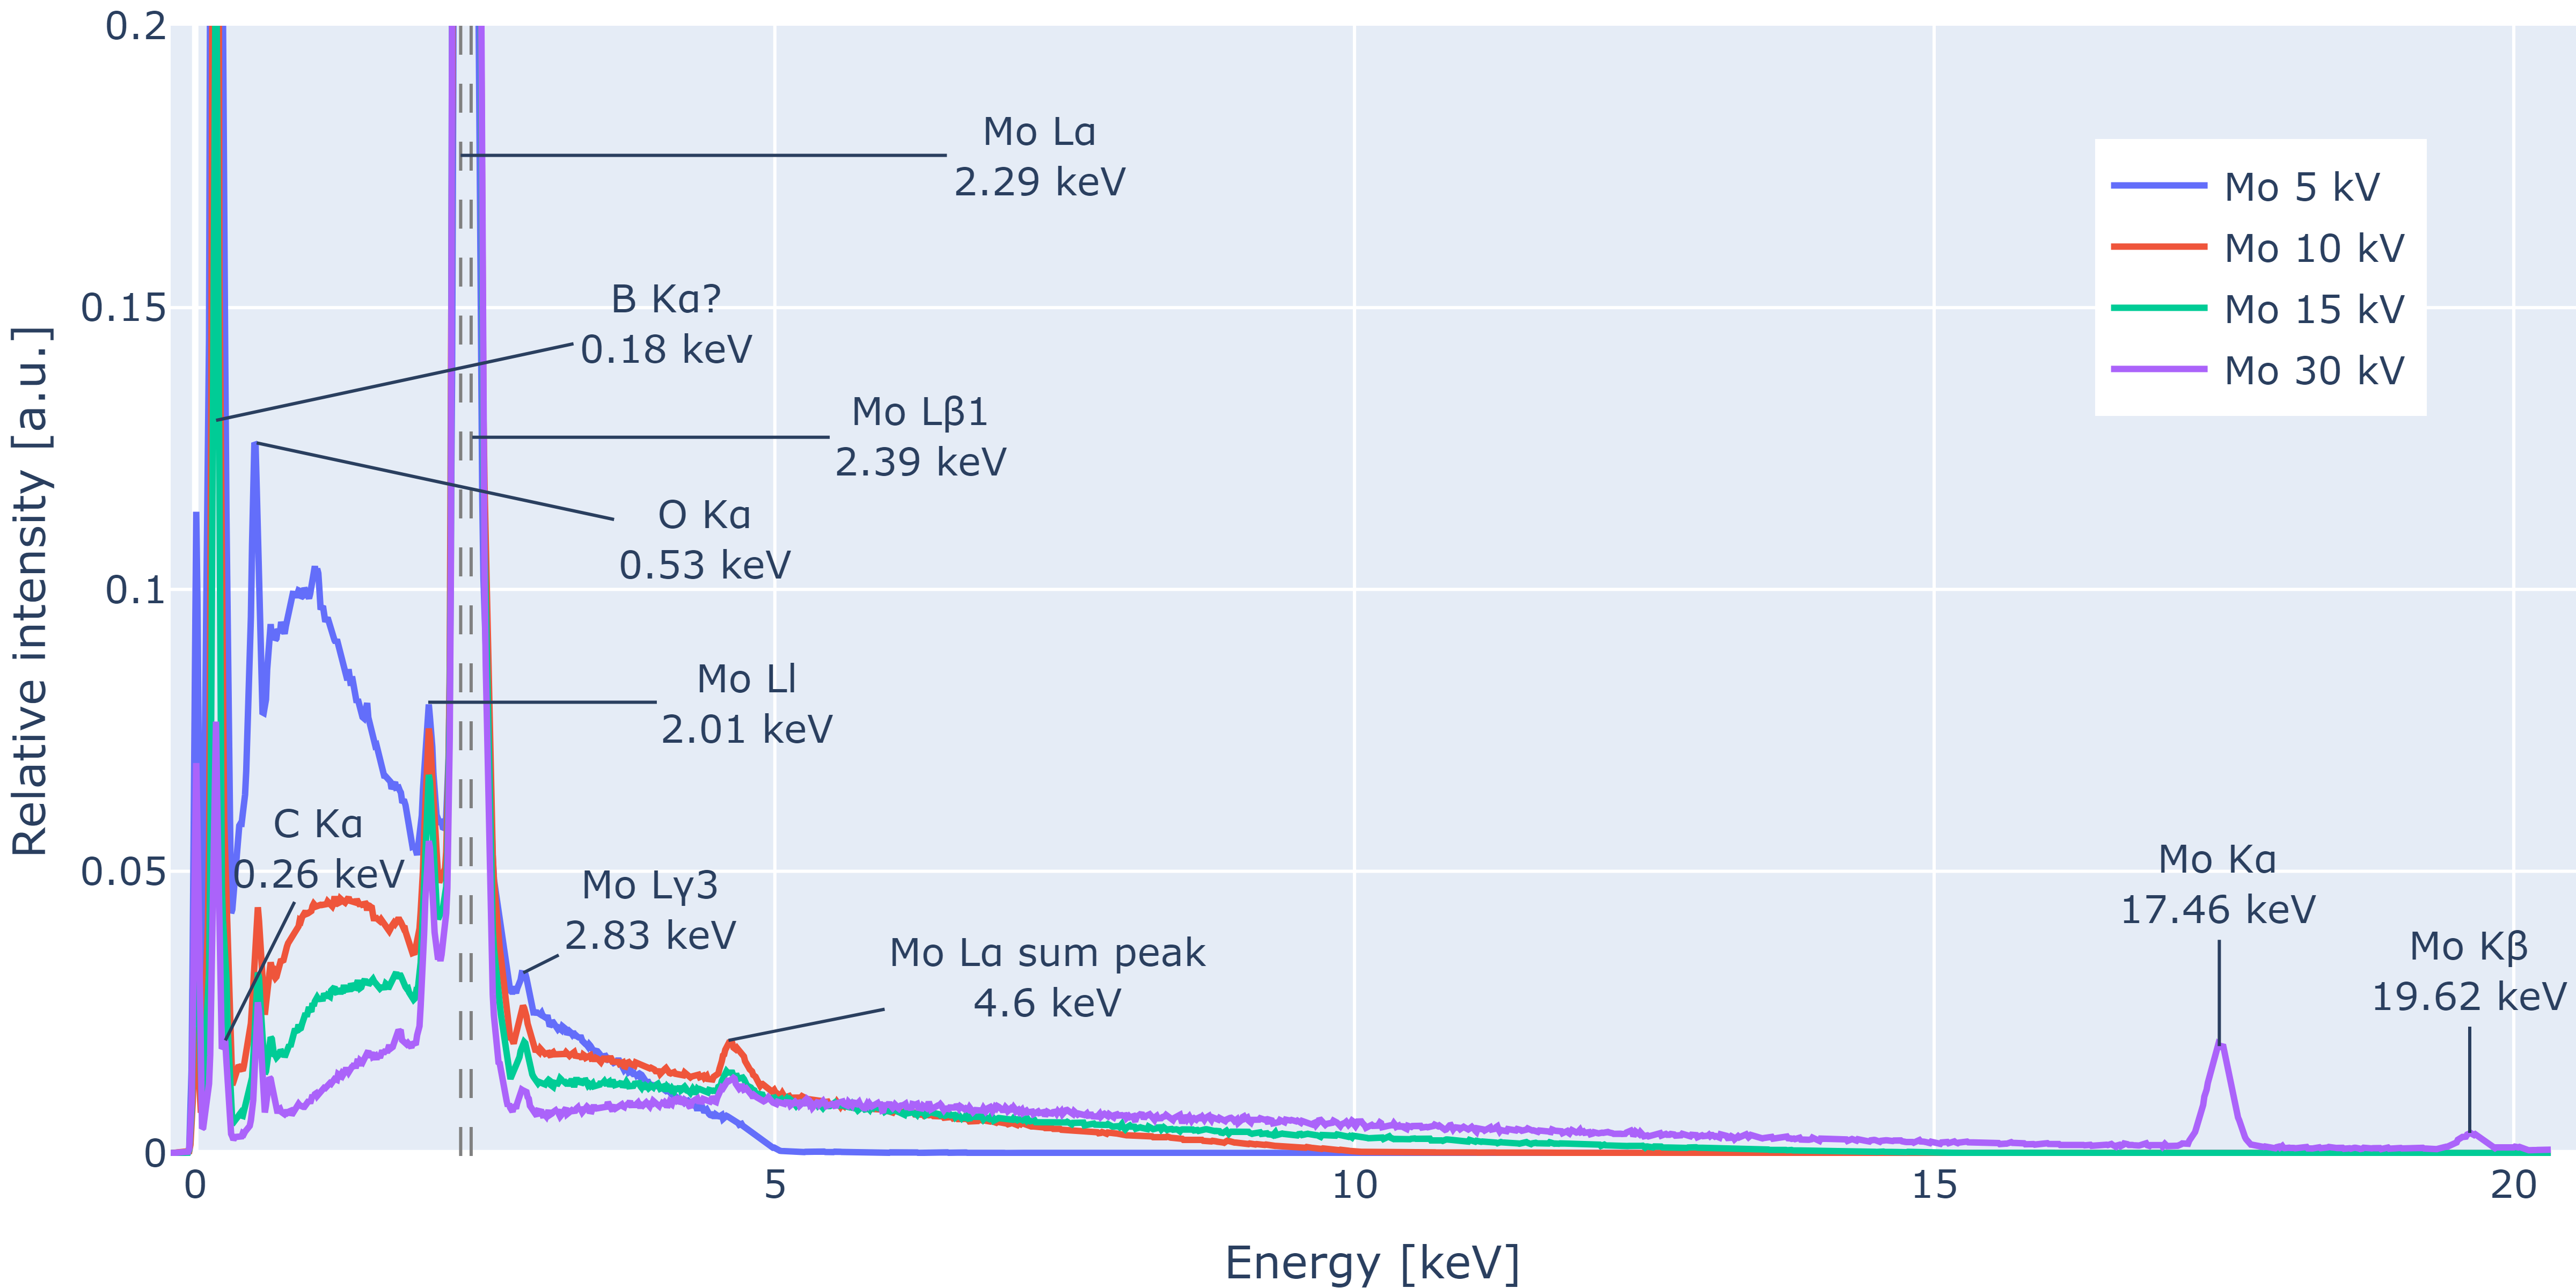
\includegraphics[width=0.90\textwidth]{../eds-analysis/plots/spectra_plots/Mo_everything.png}
    \caption{
        The spectra of the Mo sample part.
        The Mo K$\alpha$ peak at 17.47 keV is barely visible at the 30 kV spectrum, and has a high noise level.
        The high dobble peak is Mo L$\alpha$ at 2.29 keV and Mo L$\beta$ at 2.39 keV.
        In the Mo spectra the Si K$\alpha$ line is just barely visible as a very small peak, and is thus not annotated.
        The peak at 2.01 keV is the Mo Ll peak, with name and energy from the HyperSpy database.
        The peak at 2.83 keV is the Mo M$\gamma$3 peak, with name and energy from the HyperSpy database.
        Mo Ll and Mo M$\gamma$3 have weights at 0.041 and 0.011, respectively.
        The Mo L$\beta$1 peak at 2.49 keV has the weight 0.327.
    }
    \label{fig:results:Spectra_Mo}
\end{figure}

% figure Spectra_NW.png
\begin{figure}
    \centering
    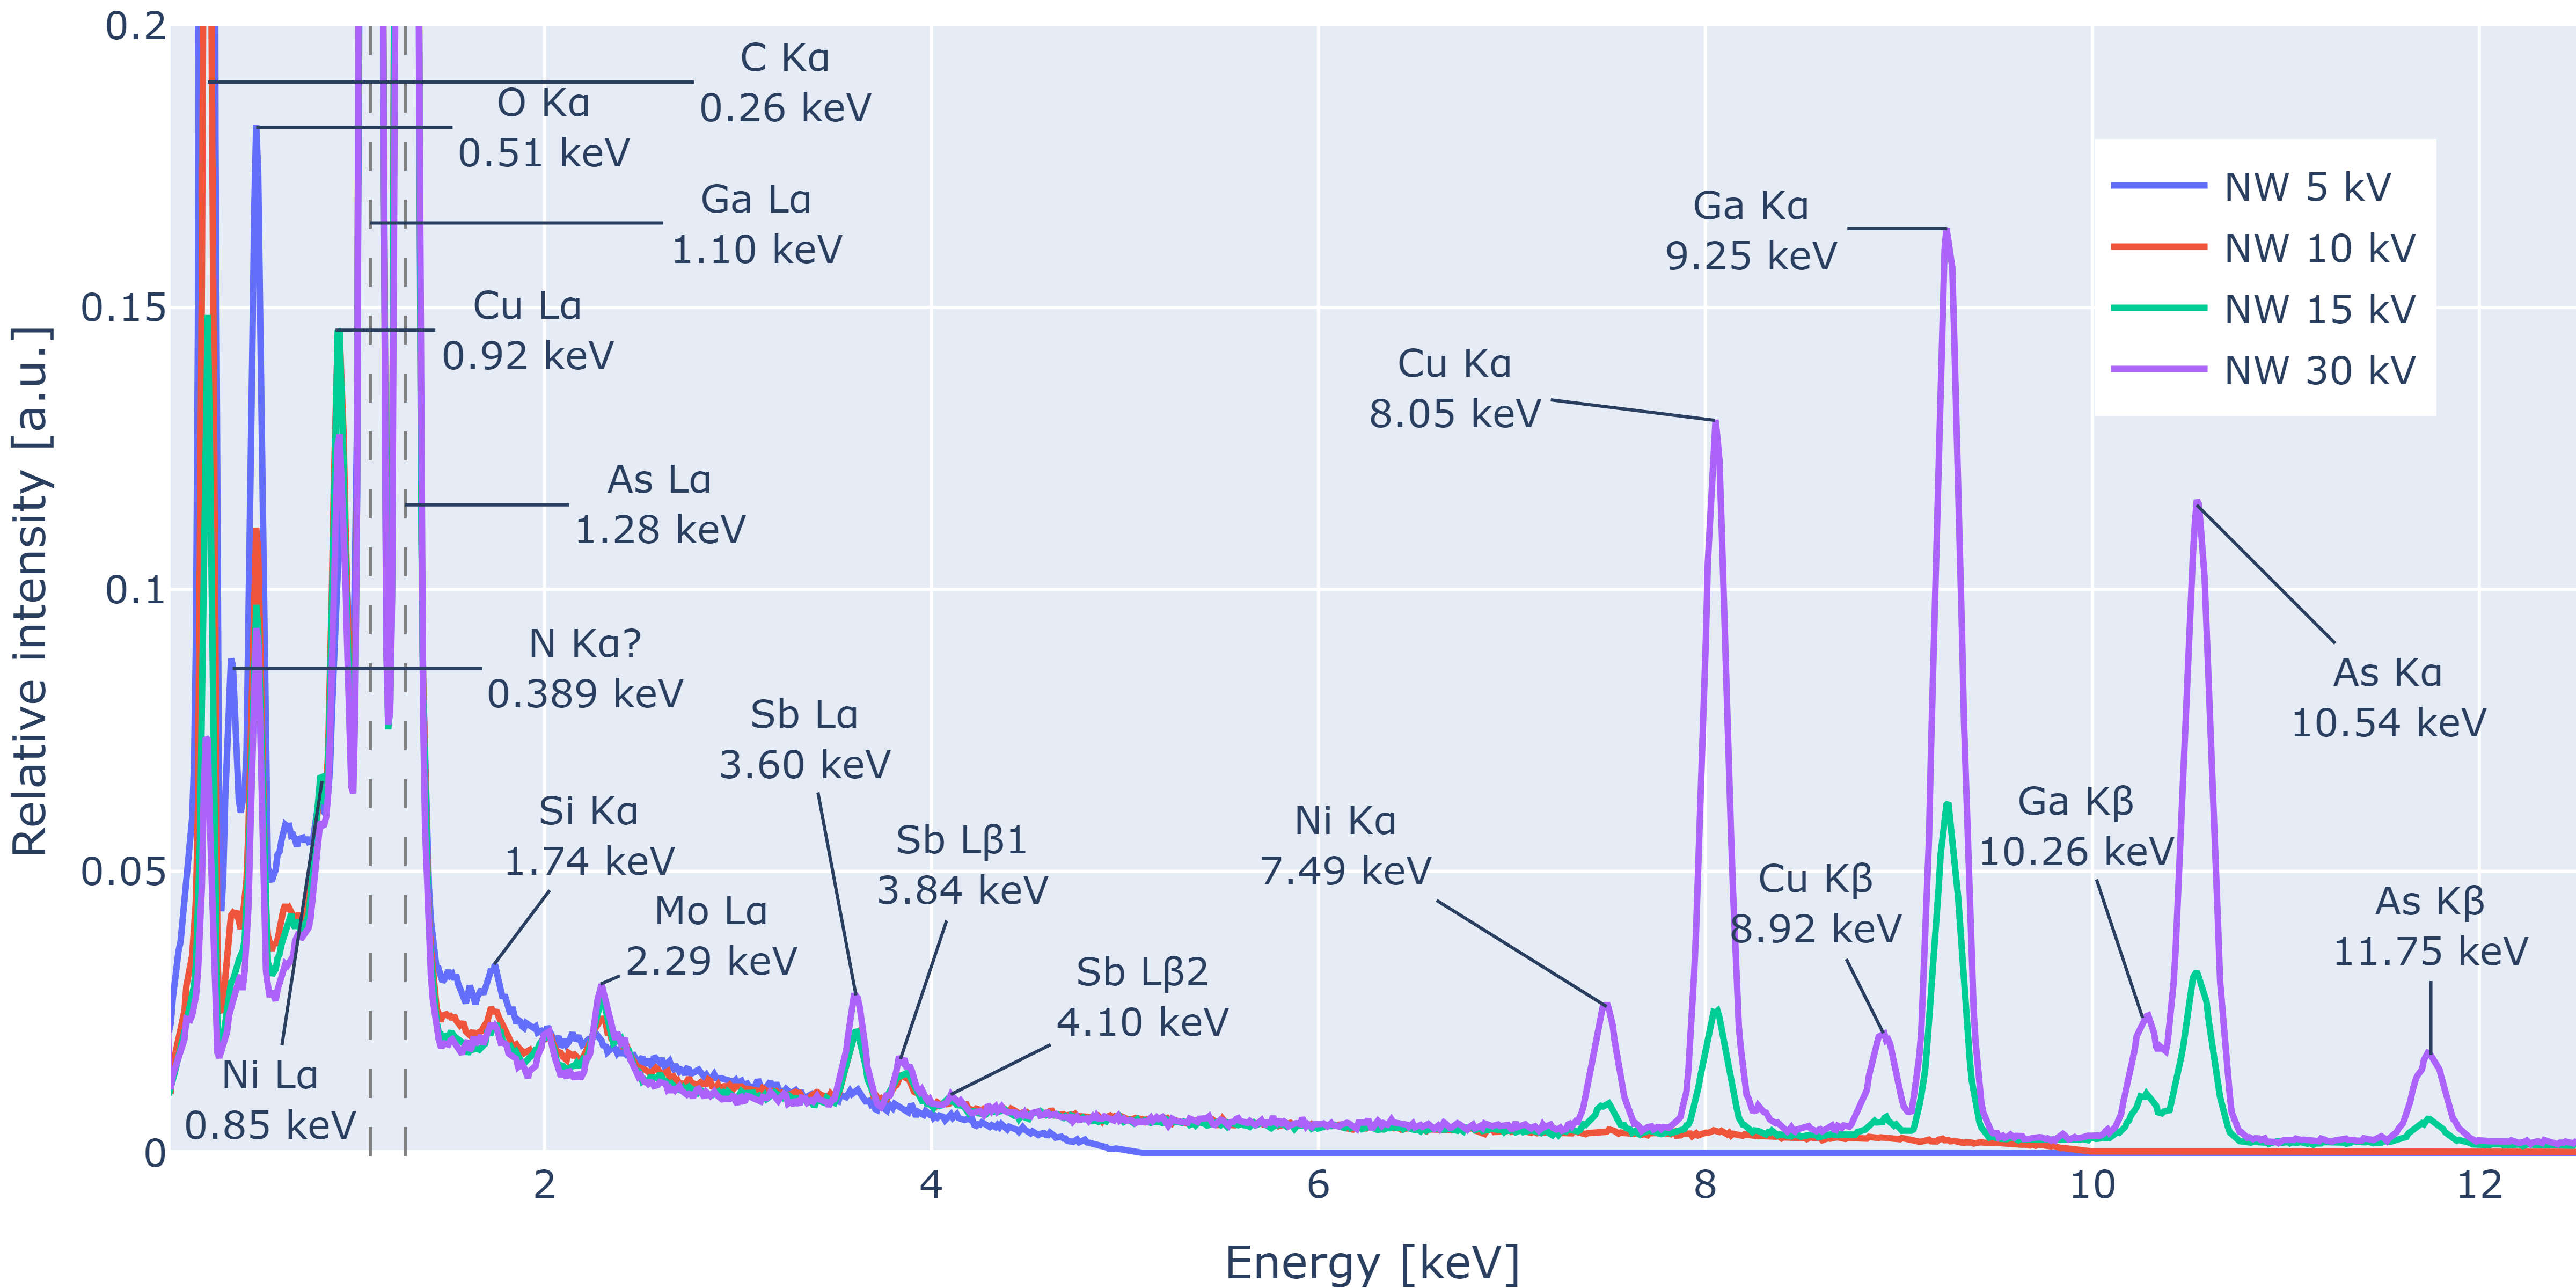
\includegraphics[width=0.90\textwidth]{../eds-analysis/plots/spectra_plots/NW_everything.png}
    \caption{
        The spectra of the nanowire sample part.
        This spectrum have the most peaks, and contains Ga, As, Cu, Sb, Mo, C, and O.
        The line at 0.389 keV could be N K$\alpha$ peak, but it could also be other elements. % Ti Ll, but no Ti K$\alpha$ peak
        The peak at 0.92 keV which is labeled as Cu K$\alpha$ is also getting a contribution from the Ga Ll peak, at 0.95 keV. % True???
        The sum peaks of the L$\alpha$ peaks are not annotated, as they are the same as in the GaAs plot, i.e. at 2.2 adn 2.4 keV.
        These sum peak are also on top of the Mo L$\alpha$ peak at 2.29 keV, and they are not distinguishable.
        The 30 kV spectrum had a small singal from the Mo K$\alpha$ peak at 17.47 keV, but that signal was weak.
        The 10, 15 and 30 kV signal have an un-annotated and un-identified peak at 2.00 keV. % what is this ???
    }
    \label{fig:results:Spectra_NW}
\end{figure}

